% Slide 3 mockup (16:9): eviction stalls the central master.
% Build: lualatex slide3_mockup.tex   (needs fig_paper_full_pool.pdf)
\documentclass{article}
\usepackage{fontspec}
\setsansfont{Helvetica}
\setmonofont{Menlo}[Scale=0.9]
\renewcommand{\familydefault}{\sfdefault}
\usepackage{graphicx}
\usepackage{tikz}
\usepackage{enumitem}
\pagestyle{empty}
\definecolor{subtext}{gray}{0.35}
\begin{document}
\setbox0=\hbox{%
\begin{tikzpicture}[x=1cm,y=1cm]
  \path[use as bounding box] (0,0) rectangle (25.4,14.29);
  \fill[white] (0,0) rectangle (25.4,14.29);

  \node[anchor=north west, font=\fontsize{21}{25}\selectfont\bfseries] at (1.0,13.5)
    {Experiment 2: Full pool. Eviction stalls lookups for 10--15\,s};

  % Figure
  \node[anchor=north west, inner sep=0] at (0.8,11.4)
    {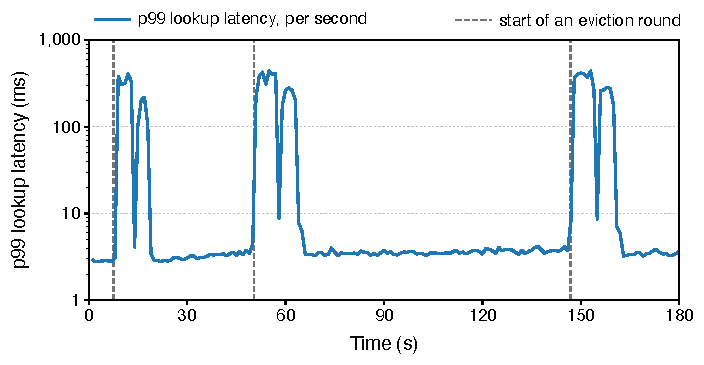
\includegraphics[width=14.6cm]{fig_paper_full_pool.pdf}};

  % Explanation
  \node[anchor=north west, text width=8.4cm, font=\fontsize{12.5}{15.5}\selectfont] at (16.2,11.6) {%
    \begin{itemize}[leftmargin=0.5cm, itemsep=9pt, topsep=0pt, parsep=0pt, label=\textbullet]
      \item \textbf{Setup.} 100M objects of 1\,MiB at the 90\% eviction watermark, so
            every write forces eviction. 16 clients write; 16 look up recent objects.
      \item \textbf{Eviction} (Mooncake defaults). Each round evicts 5\% of objects
            after scanning all keys twice, holding shard locks.
      \item \textbf{Result.} Between rounds p99 is 3.5\,ms. At each round start it
            reaches 220--440\,ms for 10--15\,s, and writes stop.
      \item \textbf{Fixable, but shared.} Incremental eviction would remove the scan;
            in a central master, any such background work still stalls every node at once.
    \end{itemize}};

  \node[anchor=south west, font=\fontsize{9.5}{11.5}\selectfont, text=subtext] at (1.0,0.7)
    {One 180\,s run; p99 per second; dashed lines: round starts from the master's log. 6\% of writes were rejected for lack of space.};
\end{tikzpicture}}%
\pdfvariable horigin=0pt
\pdfvariable vorigin=0pt
\pagewidth=\wd0
\pageheight=\dimexpr\ht0+\dp0\relax
\shipout\box0
\end{document}
